\section{OpenFace auf Video - To Do}
Durch das Lernen von OpenFace muss auch die Qualität auf einem Video betrachtet werden. Dazu wurde ein eigener Datensatz erstellt und ausgewertet.\\
Für den Versuch wurde ein Video verwendet, Welches ein Bewegtes Kreuz zeigt. Dieses Kreuz sollten die Probanden normal mit dem Blick folgen damit für jeden Zeitpunkt die Blickrichtung bekannt ist.
\subsection{Versuchsaufbau}
Die Anordnung der Eckpunkte sind in \autoref{img_targets} Dargestellt und wurden mittels eines Projektors auf eine Breite von $2.88m$ und eine Höhe von $1.49m$.\\
Das Ziel das Betrachtet werden soll (Target), beginnt immer in der Mitte und bleibt dort $1s$ Stehen, bewegt sich innerhalb von 4 Sekunden einen der Randpunkte, dargestellt in \autoref{img_targets}, verweilt dort für eine Sekunde und begibt sich in $4s$ zu einem nächstgelegenen Randpunkt, bleibt dort $1s$ und geht zurück zum Zentrum, dies wiederholt.\\
Die Versuchspersonen stellten sich etwa $1.5m$ von der vor der Leinwand entfernt auf, die Kamera befand sich $24cm$ unterhalb und $12.5cm$ vor dem Zentralen Punkt der Targets mit Blickrichtung von den Targets weg.
\begin{figure}
	\centering
	\fbox{
\includegraphics[width=0.7\linewidth]{img/Targets}}
	\caption{Eckpositionen des Bewegten Zieles bei der Videoaufnahme}
	\label{img_targets}
\end{figure}
\subsection{Versuchs - Durchführung}
Um die ungefähre Position des Kopfes zu ermitteln, wurde die Distanz zwischen dem Nasenrücken und den 4 Eckpunkten mittels eines Laserdistanzmessers bestimmt um die Position relativ zur Leinwand und Kamera zu ermitteln.\\
Während der Aufnahme wurde auf weitere Messung der exakten Position verzichtet.
Die 6 Probanden (5 Männlich, 1 Weiblich, 3 Brille, 5 Ohne) verfolgten das Ziel $2m$ und $1s$ auf natürlicher weise.\\
Um die Bewegung des Punktes mit der Aufgezeichneten Kopfbewegung zu Synchronisieren, war im Kamerabild der duplizierte Bildschirm zum Projektor zusehen.\\
Die Aufnahme wurde mit $15Fps$ in Farbe mit einer Auflösung von $1600\times 896$ Pixel aufgezeichnet. Die Kamera besitzt einen horizontalen Blickwinkel von etwa $70^\circ$.
\subsection{Ergebnis}
Die Auswertung des Versuches hat die Erwartungen und Problematiken bestätigt. Eine Verarbeitung des Videomaterials ist sogar bei sehr niedriger Auflösung noch möglich, wobei die Qualität besser sein könnte.
\subsubsection{Erster Eindruck}
Dargestellt in \autoref{img_videosumme} sind alle Auftreffpunkte der Blickrichtung auf die Leinwand währen der gesamten Aufnahme.\\
\begin{figure}
	\centering
	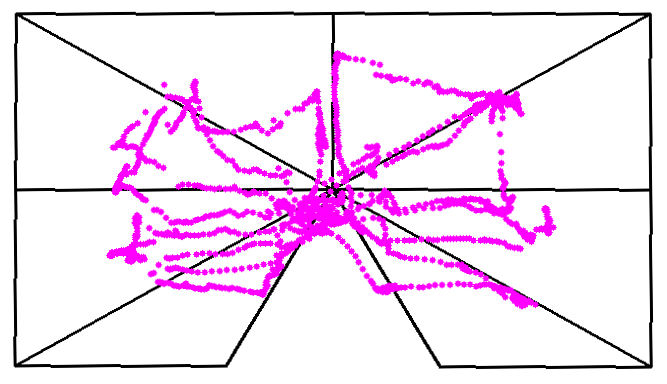
\includegraphics[width=0.7\linewidth]{OpenFace_Img/VideoSumme}
	\caption{Dargestellt sind alle gemessene Auftreffpunkte der Gesichtsorientierung auf die Leinwand (Rosa) und des Targets (Schwarz)}
	\label{img_videosumme}
\end{figure}
Es ist zu erkennen, dass die eigentlichen Bewegungen erkennbar sind, es aber vor allem in den Randbereichen zu einer großen Differenz kommt.\\
Da nur der Unterschied zwischen Target und Auftreffpunkt der gemessenen Gesichtsorientierung aufgezeigt werden kann, kommt es zu verschiedenen Fehlern, vor allem wird dem Target mit den Augen gefolgt.
\subsubsection{Qualität}
Durch die begrenzte Auflösung der Kamera und dem großen Distanzbereich auf dem gearbeitet werden muss, ist vor allem die Stabilität bei der Skalierung wichtig.
\begin{figure}
	\centering
	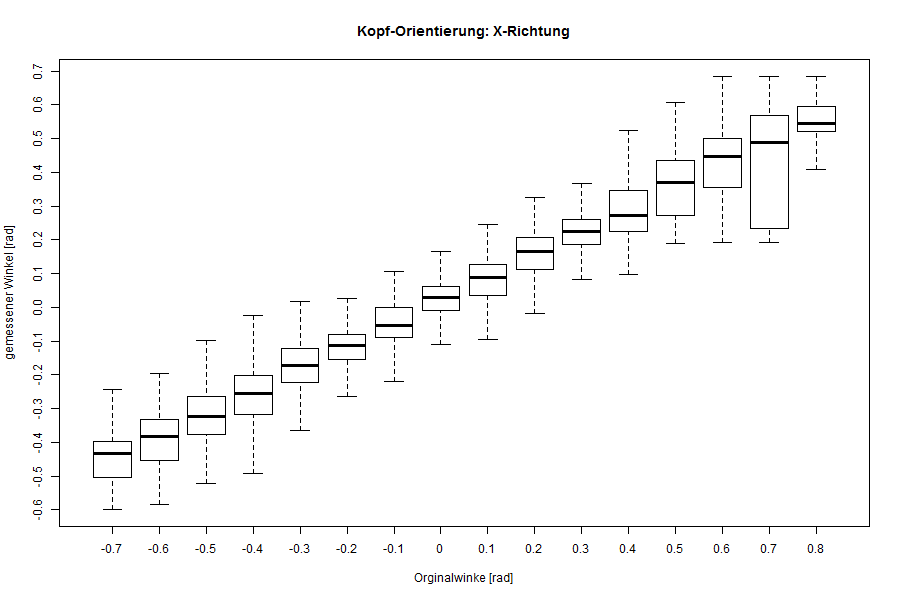
\includegraphics[width=0.3\linewidth]{OpenFace_Img/Head_x_S1}
	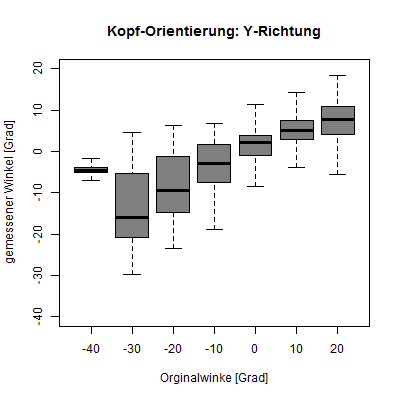
\includegraphics[width=0.3\linewidth]{OpenFace_Img/Head_y_S1}
	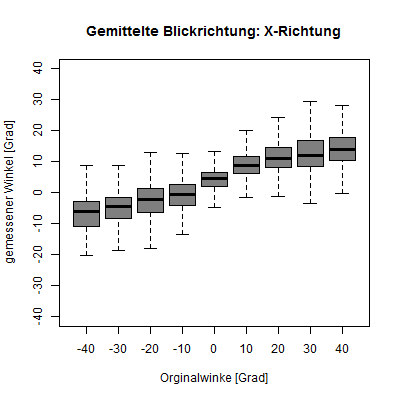
\includegraphics[width=0.3\linewidth]{OpenFace_Img/EyeAVG_x_S1}\\
	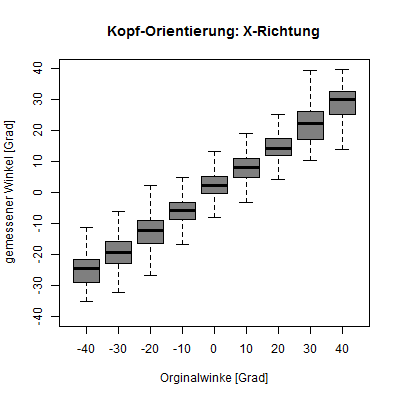
\includegraphics[width=0.3\linewidth]{OpenFace_Img/Head_x_S05}
	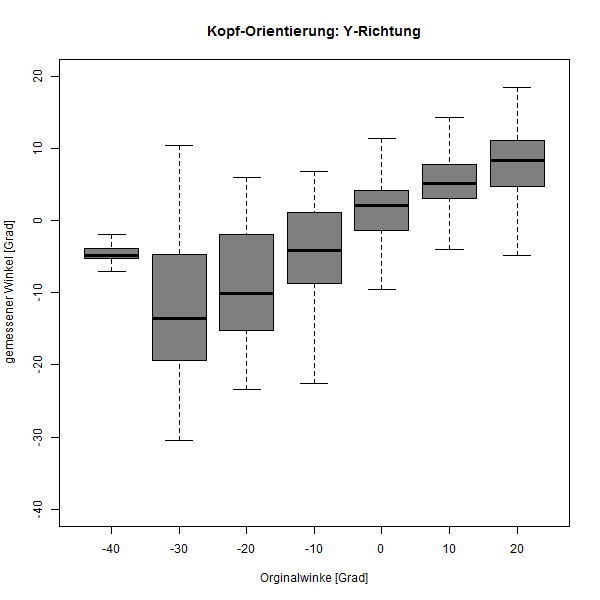
\includegraphics[width=0.3\linewidth]{OpenFace_Img/Head_y_S05}
	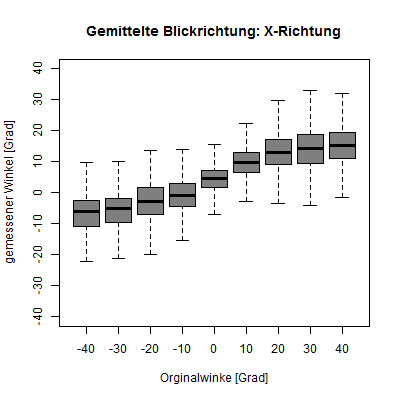
\includegraphics[width=0.3\linewidth]{OpenFace_Img/EyeAVG_x_S05}\\
	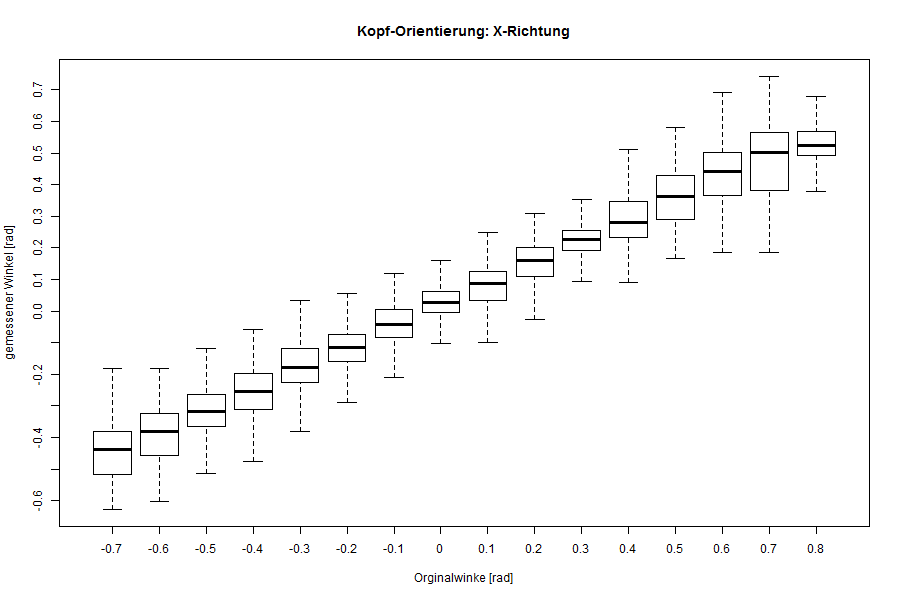
\includegraphics[width=0.3\linewidth]{OpenFace_Img/Head_x_S025}
	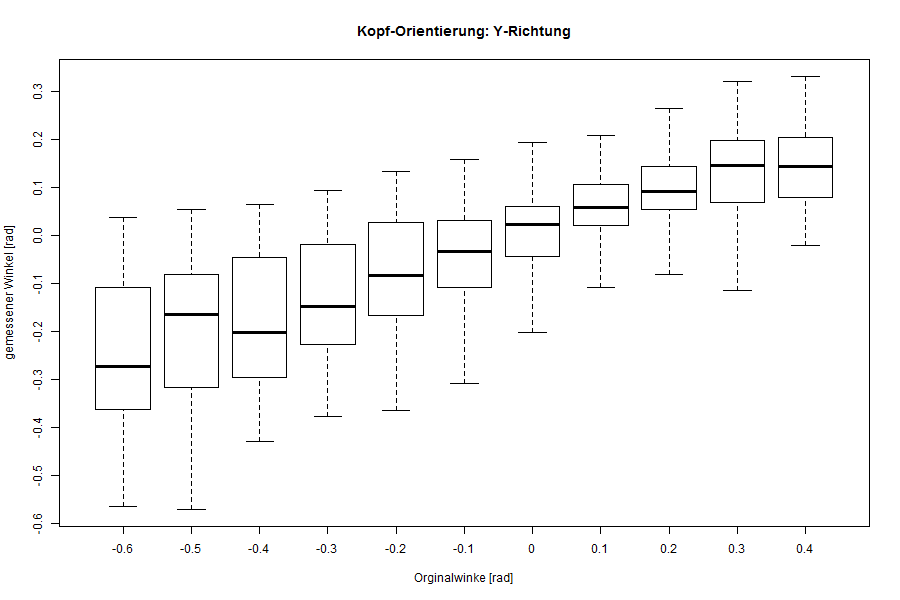
\includegraphics[width=0.3\linewidth]{OpenFace_Img/Head_y_S025}
	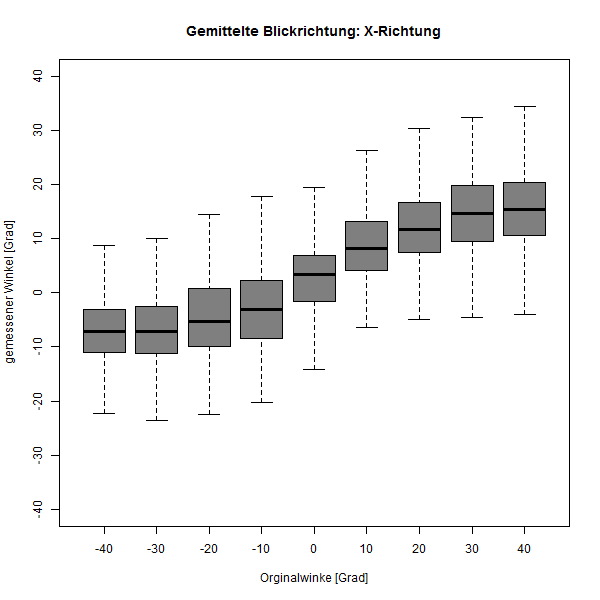
\includegraphics[width=0.3\linewidth]{OpenFace_Img/EyeAVG_x_S025}\\
	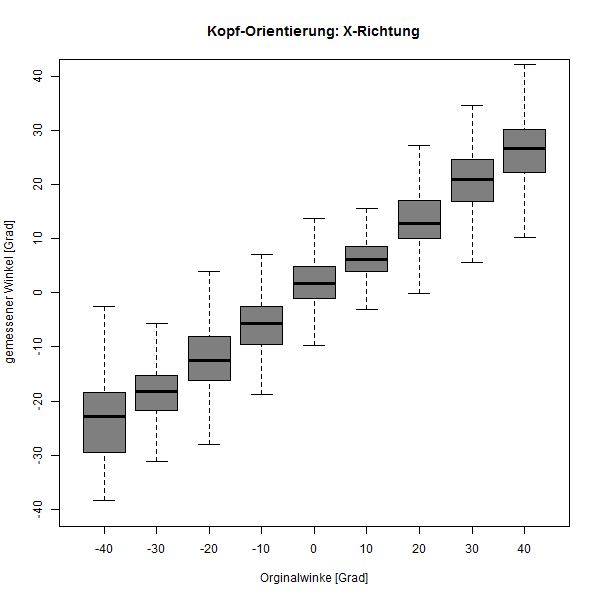
\includegraphics[width=0.3\linewidth]{OpenFace_Img/Head_x_S01}
	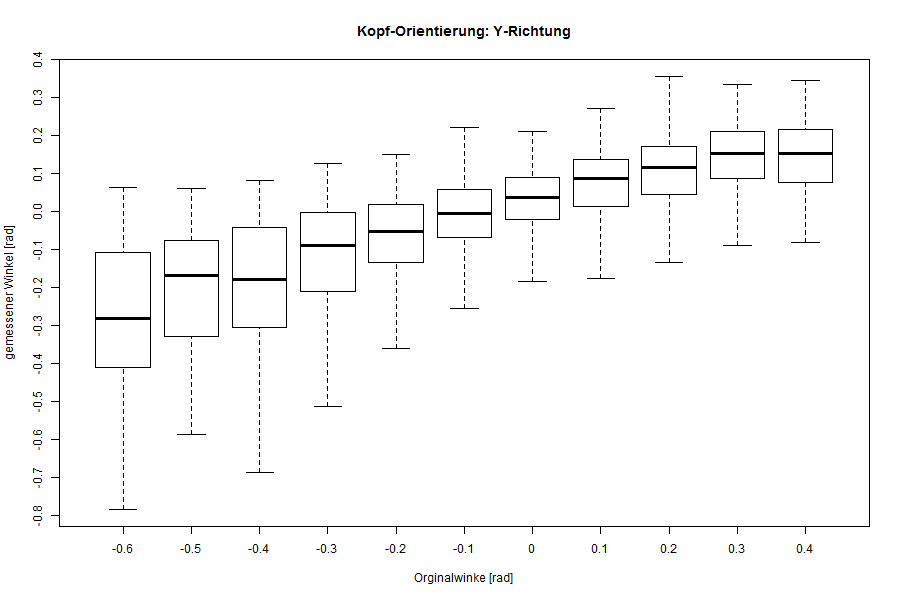
\includegraphics[width=0.3\linewidth]{OpenFace_Img/Head_y_S01}
	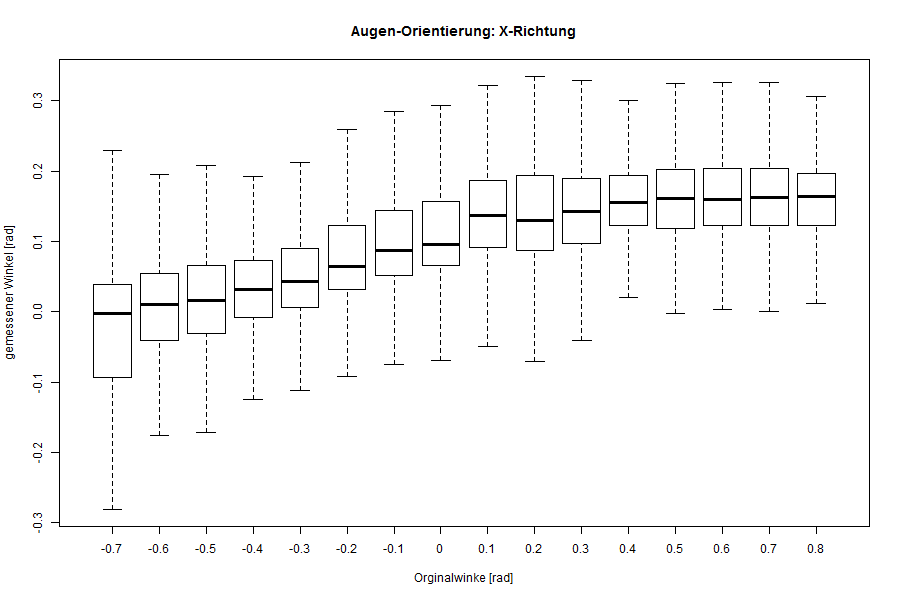
\includegraphics[width=0.3\linewidth]{OpenFace_Img/EyeAVG_x_S01}\\
	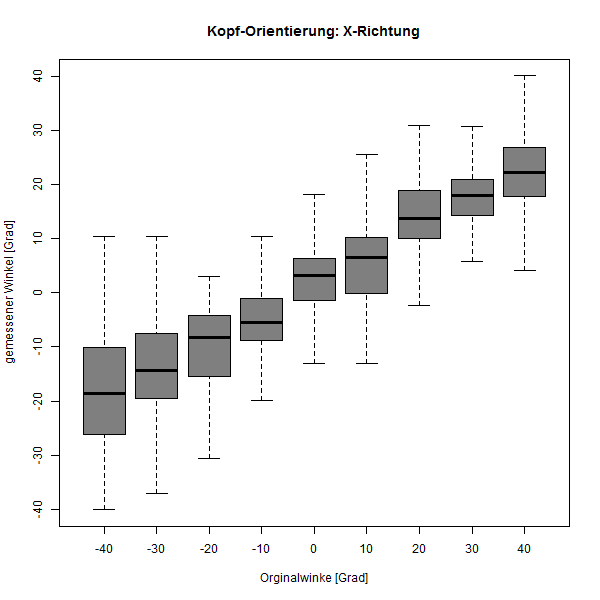
\includegraphics[width=0.3\linewidth]{OpenFace_Img/Head_x_S005}
	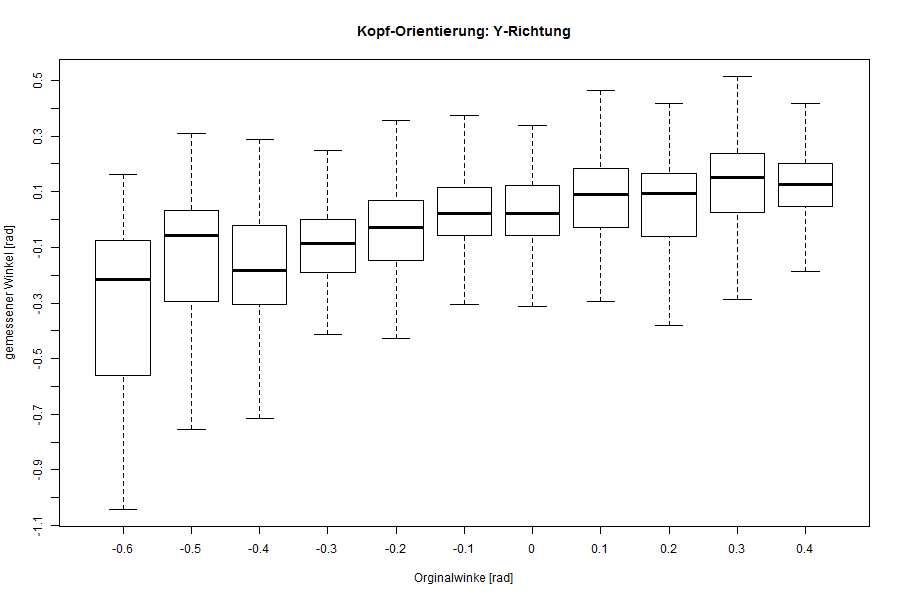
\includegraphics[width=0.3\linewidth]{OpenFace_Img/Head_y_S005}
	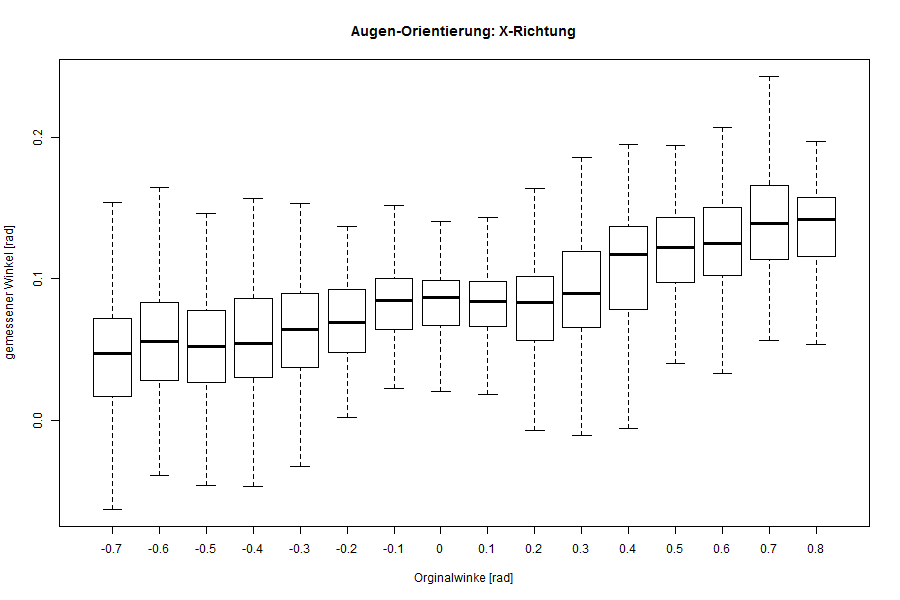
\includegraphics[width=0.3\linewidth]{OpenFace_Img/EyeAVG_x_S005}
	\caption{Dargestellt ist Auswertung der Videoaufnahme mit der Kopfausrichtung Horizontal (Links), Kopforientierung Vertikal (Mitte) und die X-Ausrichtung der Augen (Rechts)\\Skalierungsfaktor von oben nach unten (1/0.5/0.25/0.1/0.05)}
	\label{graph_VideoSkalierung}
\end{figure}
Bei der Bestimmung des horizontalen Winkels der Kopforientierung zeig sich das die bestimmten Werte im schnitt etwas zu gering ist. Der Richtung zur Kamera kann zuverlässig bestimmt werden, je größer der zu messende Winkel ist, desto  stärker wird auch der Fehler.\\
Betrachtet man die jeweiligen Quartale, so sind die Grenzen etwa $5^\circ$ auseinander in der Originalgröße. Genug um einzelne Bereiche differenzieren zu können, jedoch zu ungenau für Berechnungen.\\
Bei der Bestimmung des vertikalen Winkels zeigt sich das dieser Wert nur sehr ungenau bestimmt werden konnte, vor allem der Winkel nach Oben ist fast nicht messbar. Jener Richtung Boden wird besser erfasst, allerdings ist, bedingt durch den Versuchsausbau, der Wertebereich geringer.\\
Die bestimmte Blickrichtung ist trotz Verbesserung durch ElSe und Mittlung beider Augen, schon in der Originalgröße nicht verwendbar. Die Mittelwerte liegen selbst bei den Maximal Werten sehr eng beieinander und die Bereiche überschneiden sich stark. Die Differenz der Mittelwerte von den Extremar sind nur etwa $20^\circ$ auseinander liegen, bei einer eigentlichen Differenz von etwa $90^\circ$.\\
Die Auswirkung der Skalierung ist annehmbar gering, allgemein steigt die Abweichung und der Bereich sinkt. Bei einem Skalierungsfaktor von 0.01 können die einzelnen Bereiche noch gut getrennt werden, dies entspricht eine Distanz von etwa $14m$. So liegt der Abstand der Quartale etwa $9^\circ$ weit auseinander auf der horizontalen Achse.\\
Bei der Bestimmung des vertikalen Winkels ergibt sich ein ähnliches Verhalten, wobei vor allem der Wertebereich auch $30^\circ$ sinkt.\\
Das Ergebnis der Blickrichtung kann nicht verwendet werden, da die Differenz zwischen dem Rechten und Linken Maximalwert nur $8^\circ$ beträgt und die Quartale sich fast vollständig überschneiden.\\
Überraschend ist das Ergebnis bei dem Skalierungsfaktor von 0.05 (ca $24m$). Die Ausrichtungen sind, zumindest horizontal, noch erkennbar und soweit differenzierbar um grobe Richtungsänderungen zu erkennen. 
\subsection{Fehleranalyse}
Eine Betrachtung der Fehlerquellen die Bei der Messung entstanden sind bzw. die durch den Aufbau Entstehen. Außerdem eine weitere bei der Berechnung.
\subsubsection{Messung}
Die erste Ungenauigkeit liegt bei der Distanz zur Leinwand, diese wurde nur zu beginn, vor der eigentlichen Aufnahme bestimmt. Somit ist entsteht eine Abweichung da Kopf in Bewegung ist, auch währen der Aufnahme.\\
Die eigentliche Messung der Distanz ist ebenfalls ungenau, da sie eine Abweichung von etwa $1cm$ in alle Richtungen aufweist. Außerdem liegt der Ursprung der Rechnung etwas Tiefer und weiter Hinten als der Messpunkt.
Die Parameter für der Überführungsmatrix von Welt- nach Kamerakoordinaten sowie die Brennweite wurden zwar sorgsam bestimmt, sind aber dennoch nicht perfekt.\\
Durch den Bedingten Aufbau, musste die Kamera in Richtung des Projektors ausgerichtet werden, wodurch diese wiederum von dem direkten Licht geschützt werden musste. Somit konnte sich die Kamera nicht im Zentrum der Messpunkte befinden.\\
Da die Kamera und die Leinwand fest Montiert sind, ergibt sich auch die Problematik das der Kopf der Probanden ebenfalls nicht im Zentrum des Kamerabildes Befinden und somit immer ein Blickwinkel von unten auf das Gesicht entsteht.\\
Da die Probanden ebenfalls zwischen der Leinwand und dem Projektor standen, verdeckten diese das Bild, wodurch es manchmal passierte das der Zielpunkt im Schatten verschwand.
\subsubsection{Umgebung}
Bei der Aufzeichnung hat sich vor allem das Problem mit der ungleichmäßigen Beleuchtung bzw. dem Gegenlicht ergeben. Diesem musste entgegengewirkt werden, damit das Gesicht gut erkennbar ist. Ein Problem das auch in der realen Anwendung auftreten wird.\\
Ein weiteres allgemeines Problematik zeigt sich auch wieder bei der Auflösung des Gesichtes, somit ist eine Berechnung auf dem Gesicht zwar möglich, auf den Augen allerdings nicht.\\
Somit ergibt sich ein weiteres Problem, da im allgemeinen eine Exkursionen, der Winkelbereich der Augenbewegungen, bis etwa  $20^\circ$ stattfindet und diese nicht erfasst werden können.\\
Ein Weiterer nicht zu verachtendes Problem ist die Ruflektion vor allem auf den Brillen, von den starken Lichtquellen wie Fenster, Projektor- und dessen Bild sowie der Lampen. Auch Schatten gerade bei den Augenhöhlen erschweren die Auswertung. 
\begin{itemize}
	\item Bild für den Versuchsaufbau
	\item Typ der Kamera
\end{itemize}
